\documentclass[12pt]{article}
\usepackage[utf8]{inputenc}
\usepackage{graphicx}
\graphicspath{{images/}}
\begin{document}
\begin{center}
\huge\underline{``Future Of Healthcare''}
\end{center}
\begin{center}
 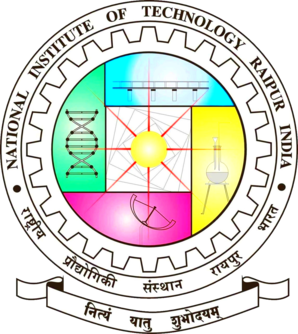
\includegraphics[scale=0.8]{nitlogo.png }
\end{center}
\vspace{1cm}
\begin{center}
   \emph{\large By}\\
\Large{Raj Motwani }\\
\large{Roll No- 21111042}\\
\large{Biomedical 1st Sem}\\
\end{center}

\newpage
\huge{\underline{Nanotechnology in future medical}}
\large
\\
In the 1966 sci-fi classic Fantastic Voyage, a submarine and its crew is shrunk to microscopic size and injected into the human body. Thecrew's mission is to repair a blood cot in the brain of an inured scientist.
While we may not be able to shrink human doctors down to microscopic size today, medicine on an atomic and molecular scale is fast becoming reality. The 2016 Nobel Prize in chemistry was awarded to a trio of scientists for the design and synthesis of molecular machines -
molecules with controllable movements - and in their recognition, the Swedes acknowledged the momentous potential of a field still in its
intancv.
Materials at the nanoscale - in the tens of nanometers - are almost incomprehensibly tiny a sheet of paper is about 100,000 nanometers thick). Engineering at this size requires manipulating individual atoms. Physical properties, such as conductivity or melting point, behave differently, making it exceptionally challenging to work with. But gaining the ability to do so - to build molecule-sized machines that car build and manipulate their environment at an autonomic level, or manipulate structures made of proteins or DNA - would be the most
radical transformation of healthcare in centuries.
Ever-smaller wearable devices that can monitor our vital signs are becoming common, but at a nanoscale we could implant them into
our bodies. Nano devices could capture incredibly detailed data from deep within us, enabling doctors to personalise treatment. Indeed
innovators in the field are working on this already: Proteus Digital Health, for instance, an Anglo-American firm named after the Fantastic
Voyage submarine, has developed ingestible sensors that fit inside pills and report in real-time from within the body.
When they reduce further to the nanoscale, such technology would radically improve medical imaging by delivering molecular resolution.
Micro machines could identify and destroy cancer cells, keeping healthy cells untouched. They could also deliver dopamine directly to
the brainstem to help treat sutterers of Parkinson's. With nanorobots, we could enter the body and even redesign the genome.
We can even imaaine autonomous nanorobots that eventuallv swim deep inside us. detectina and reactina to problems as thev arise
Looking back on Fantastic Voyage, it seems reality could one day exceed even the most imaginative science fiction.

\huge{\underline{``IOT in Healthcare''}}\par
\Large
We can consider an IoT unit as a device with a sensor that can interact with the physical world and send information to the Internet. All these Iot based healthcare devices can communicate with each other to take important actions that would provide timely help or even save a life.

After collecting passive data, IoT healthcare devices would send this critical information to the cloud so that doctors can act upon it. Thus, IoT-based healthcare services not only improve a patient’s health and help in critical situations but also the productivity of health employees and healthcare organizations’ workflows.

The rise of IoT is exciting for everybody due to its different scope of use in various sectors. In Healthcare it has several applications. Here are some remarkable IoT applications in healthcare:
Hearables , Ingestible sensors,Moodables,Computer vision technology,Insulin Pens and Smart CGM etc.

\underline{Conclusion}

IoT changes the way the facilities are delivered to the healthcare industry. These technologies improve the product, causing a larger effect by bringing together minor changes.









\enddocument